\documentclass{beamer}
\usetheme{Warsaw}

% The subfolder containing the images
\usepackage{graphicx}
\graphicspath{{Images/}}
\DeclareGraphicsExtensions{.jpg}

\title{Basic Soldering Workshop}
\subtitle{PTH and large pitch SMT}
\author{Ethan Harstad \and Ian McInerney}
\institute{
	Make to Innovate\\
	Dept. of Aerospace Engineering\\
	Iowa State University
}
\date{28 September 2013}


%\AtBeginSection[] {
%	\begin{frame}[t, shrink]
%		\frametitle{Outline}
%		\tableofcontents[currentsection]
%	\end{frame}
%}

\begin{document}

\begin{frame}[plain]
	\titlepage
\end{frame}

\section{Introduction}
\begin{frame}[t]
	\frametitle{Introduction}
	In this workshop you will learn:
	\begin{itemize}
		\item Safety hazards associated with soldering
		\item Safety precautions to take while soldering
		\item How to solder through-hole components
		\item How to solder large pitch surface mount components
	\end{itemize}
\end{frame}

\section{Safety}
\subsection{Hazards}
\begin{frame}[t]
	\frametitle{Hazard - Burns}
	A soldering iron reaches temperatures easily capable of burning the skin on contact.
	Burns can also occur through secondary means:
	\begin{itemize}
		\item Conduction of heat through working materials
		\item Contact with molten soldering constituents
		\item Ignition of secondary materials
	\end{itemize}
\end{frame}
\begin{frame}[t]
	\frametitle{Hazard - Lead Exposure}
	Lead is a known neurotoxin and is contained in many types of solder. Soldering temperatures are not capable of producing lead fumes and skin contact is mostly harmless. Ingestion of lead contaminants on the skin or under the fingernails still presents a major hazard. Lead is a cumulative poison that is not normally excreted from the body.\\
	Washing the hands with soap and water after soldering is sufficient protection from the effects of lead.
\end{frame}
\begin{frame}[t]
	\frametitle{Hazard - Fumes}
	Hazardous fumes can be produced by both soldering components and surface contaminants of the solder joint. Fumes can cause irritation of the eyes, mucous membranes and respiratory tract. To avoid exposure:
	\begin{itemize}
		\item Work in a well ventilated area
		\item Keep your head to the side of the work area to avoid breathing fumes
		\item Use a fume extractor if necessary
	\end{itemize}
	Individually investigate the hazard of any chemicals used. Ask a lab monitor if unsure.
\end{frame}
\begin{frame}[t]
	\frametitle{Hazard - Skin Irritation}
	Some chemicals, such as activated fluxes, can cause skin irritation. Washing any areas of contact after soldering is usually sufficient to prevent irritation from chemicals stocked in the lab.\\
	You may wear gloves and/or long sleeves if you have sensitive skin.\\
	\textbf{Do not use any other products without prior approval.}
\end{frame}
\begin{frame}[t]
	\frametitle{Hazard - Electrocution}
	The soldering iron can provide a path for electrical current capable of electrocuting 
	the user. Never attempt to solder a circuit that is energized. Circuits with large 
	capacitors can remain energized for several minutes.\\
	\textbf{Soldering irons with a ground plug offer increased safety.}
\end{frame}

\subsection{Personal Protective Equipment}
\begin{frame}[t]
	\frametitle{Personal Protective Equipment}
	Safety glasses must be worn at all times while soldering. Solder or other components 
	used while soldering can 'spit' and damage the eyes. Cutting wire can also cause 
	fragments to fly and damage the eyes.
\end{frame}

\subsection{Safety Procedures}
\begin{frame}[t]
	\frametitle{Safety Procedures}
	\begin{itemize}
	\item Always wash your hands after soldering and before breaks.
	\item Always replace the soldering iron in the stand. \textbf{Do not lay it on the work surface.}
	\item Do not attempt to catch a falling iron.
	\item Only work over a stable work surface. Falling solder can cause burns.
	\end{itemize}
\end{frame}

\section{Basic Procedure}
\subsection{Soldering Iron Controls}
\begin{frame}[t]
	\frametitle{Soldering Iron Controls}
	\center
	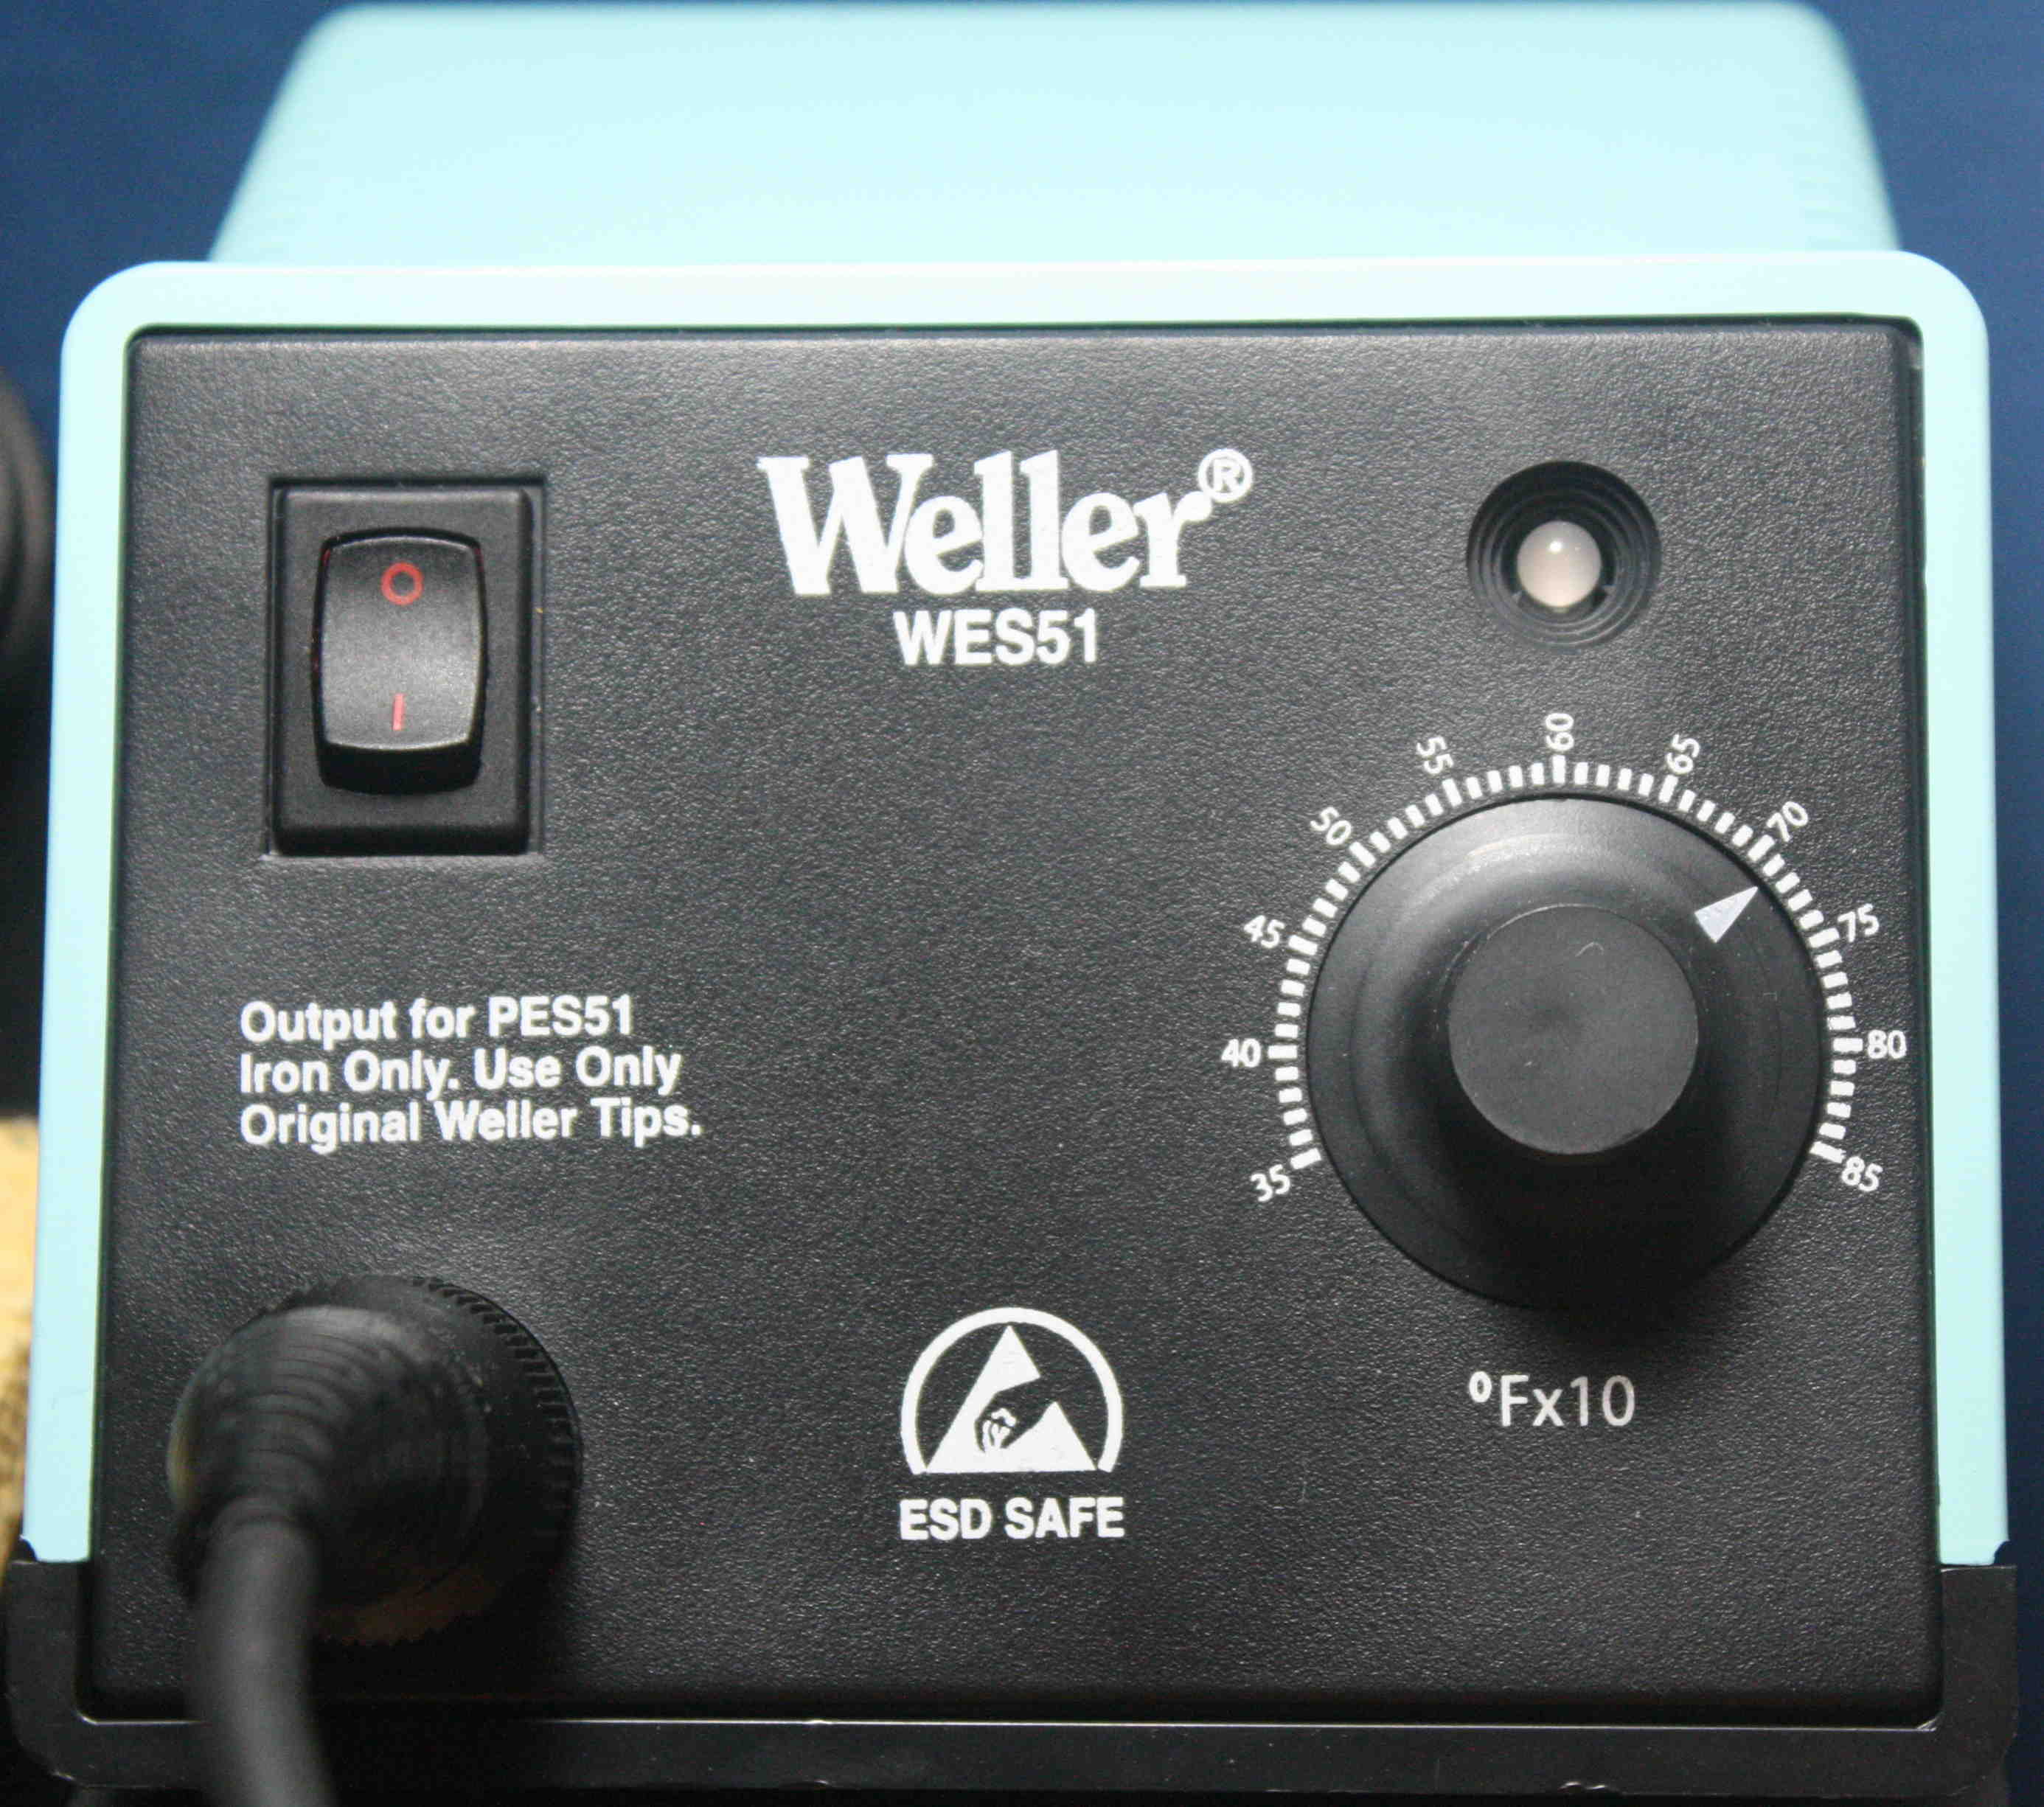
\includegraphics[height=1.5in]{WellerFront} \\
	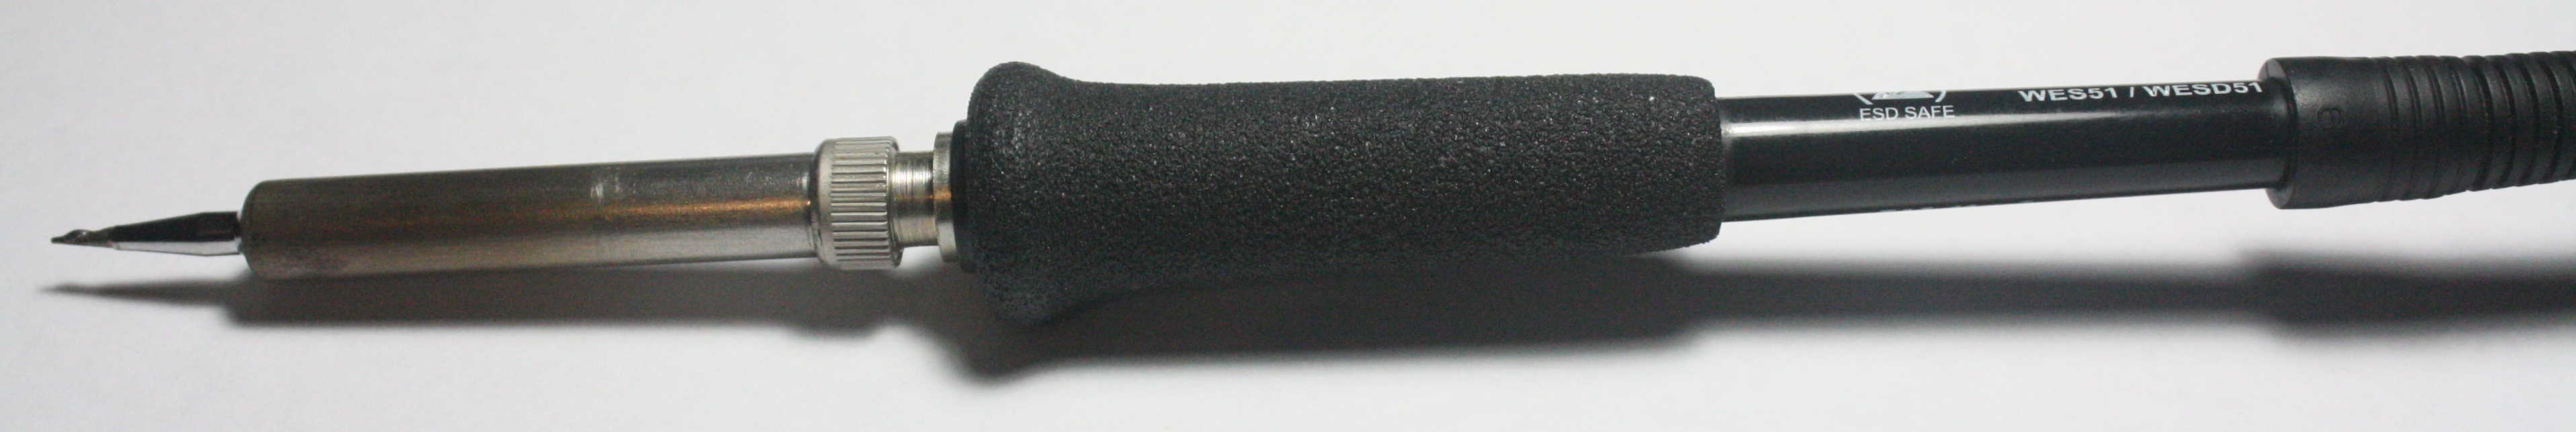
\includegraphics[width=4in]{Pencil}
\end{frame}

\subsection{Tip/Temperature Selection}
\begin{frame}[t]
	\frametitle{Tip/Temperature Selection}
	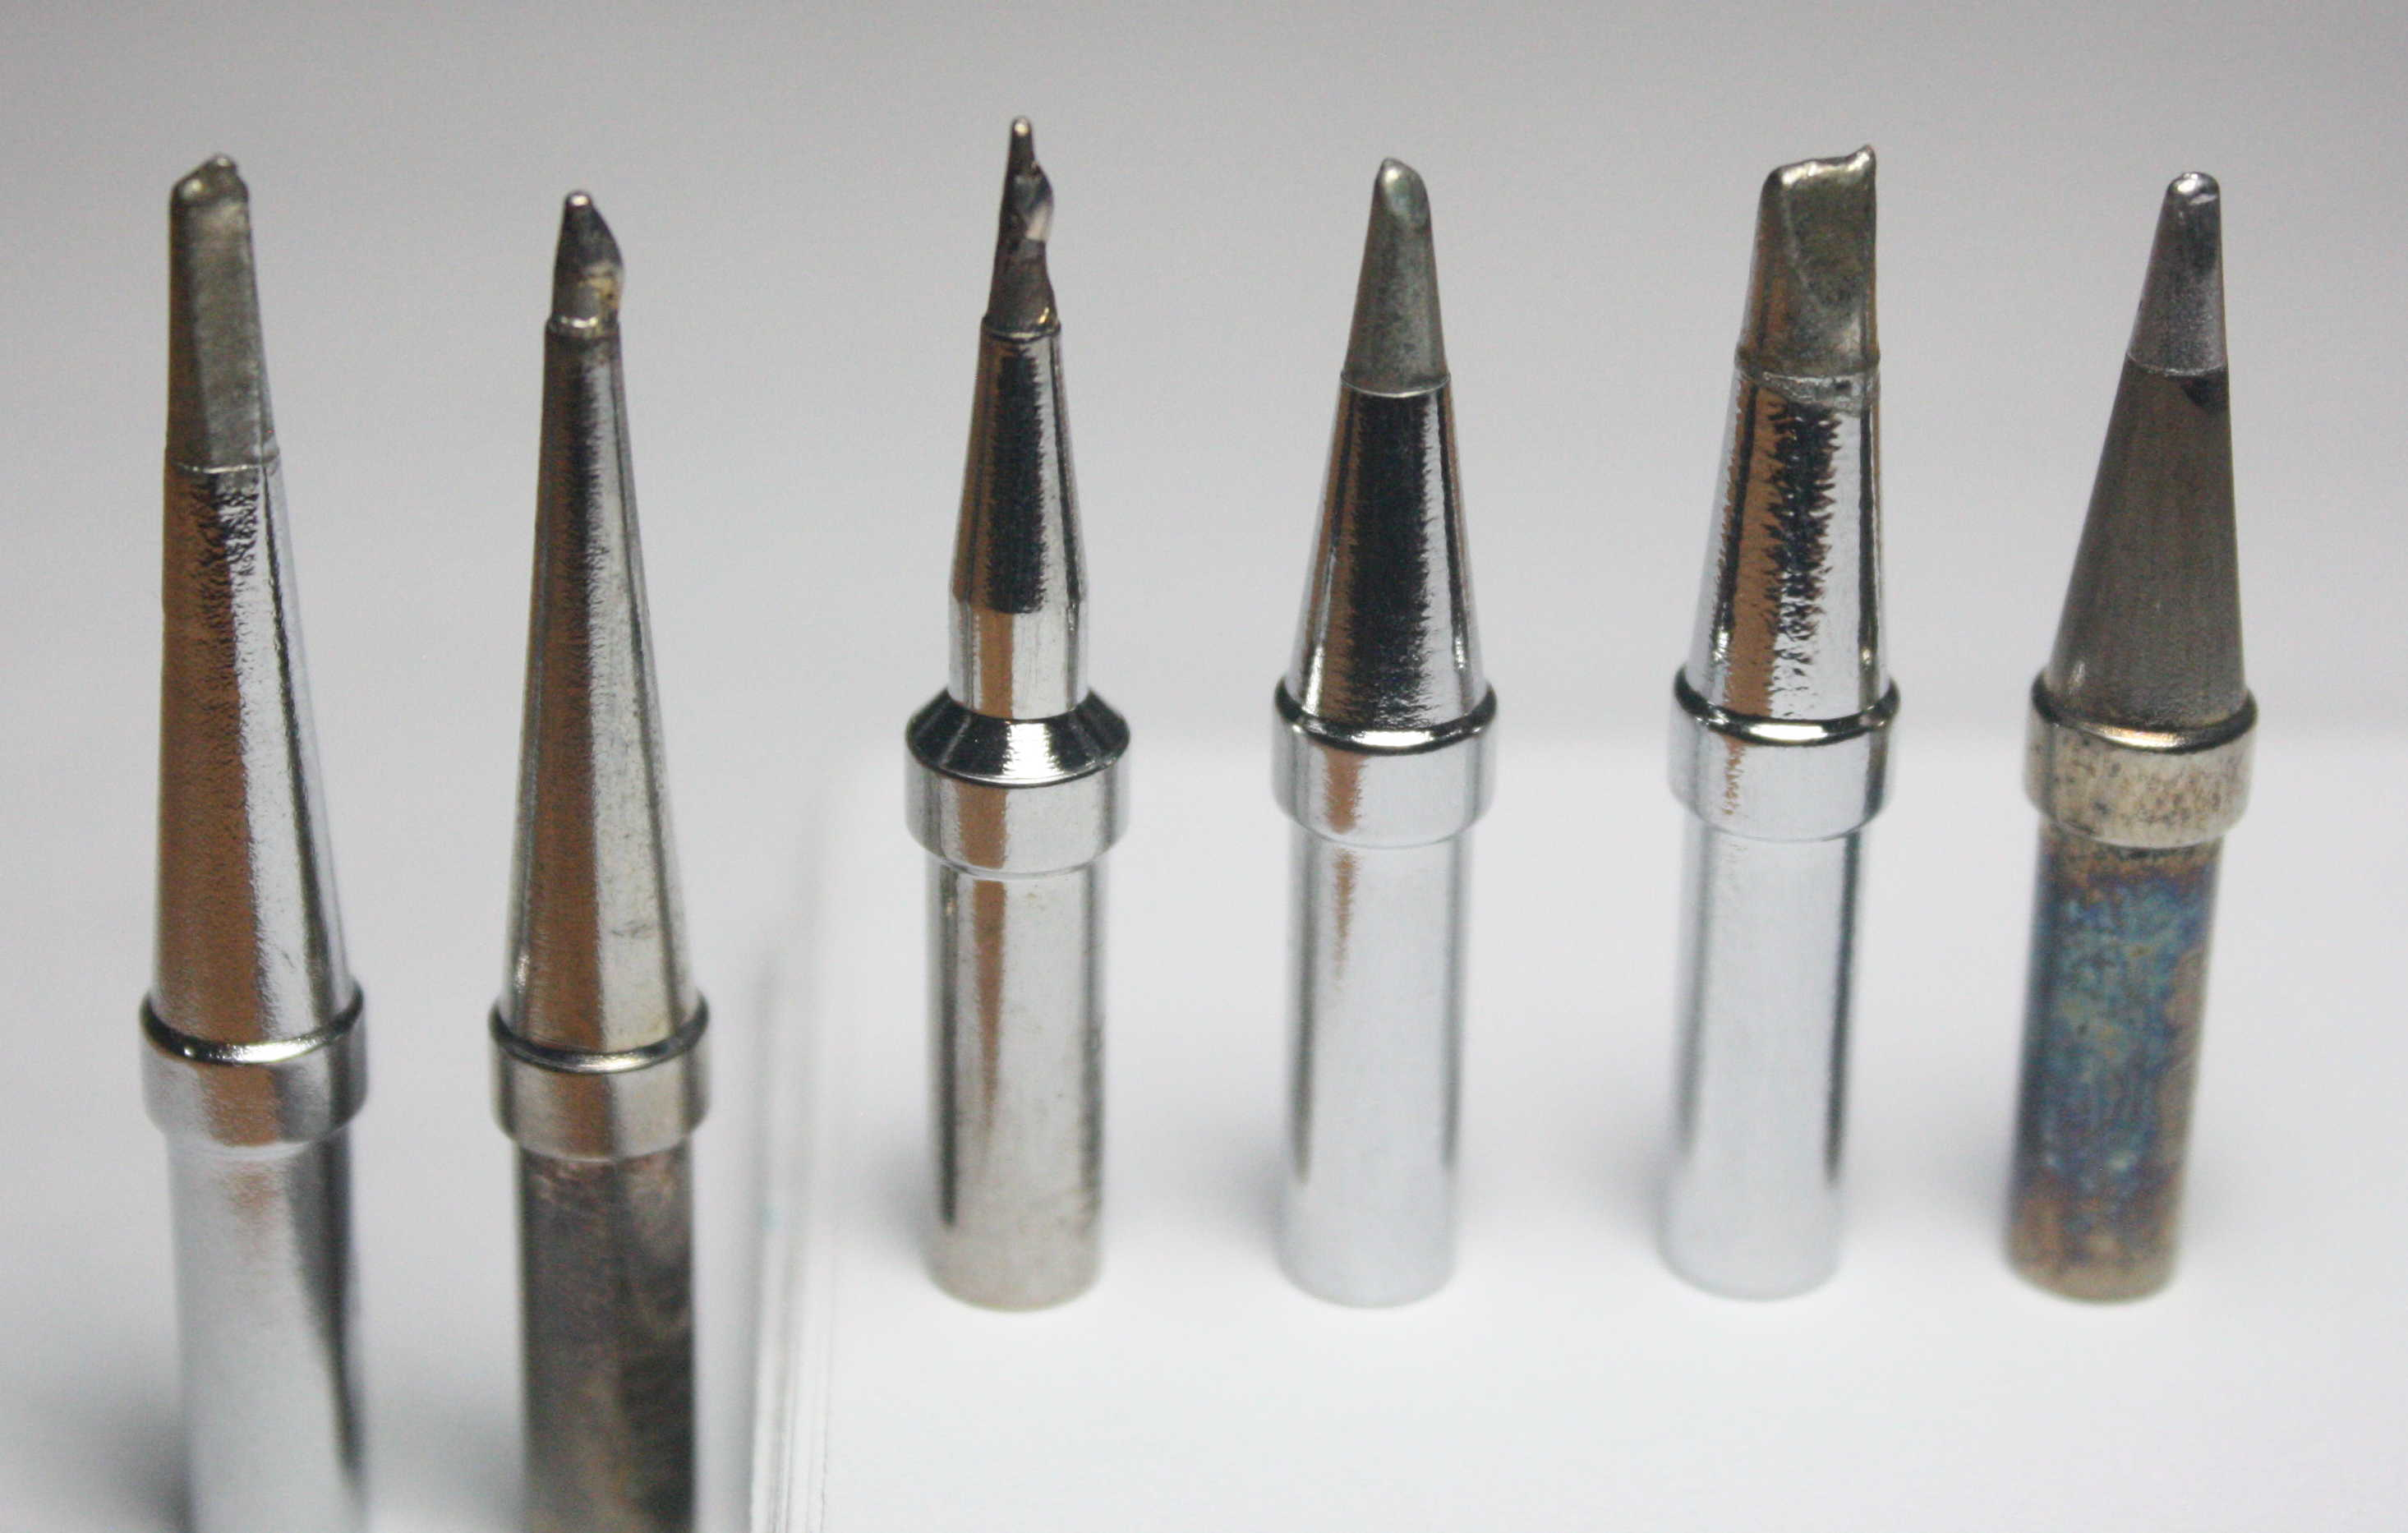
\includegraphics[width=3in]{IronTips}
\end{frame}

\subsection{Joint Preparation}
\begin{frame}[t]
	\frametitle{Joint Preparation}
\end{frame}

\subsection{Tip Preparation}
\begin{frame}[t]
	\frametitle{Tip Preparation}
\end{frame}

\subsection{Soldering}
\begin{frame}[t]
	\frametitle{Soldering}
\end{frame}

\subsection{Troubleshooting}
\begin{frame}[t]
	\frametitle{Troubleshooting}
\end{frame}

\section{Example Cases}
\subsection{Wire to Pin}
\begin{frame}[t]
	\frametitle{Wire to Pin}
\end{frame}

\subsection{Wire to Wire}
\begin{frame}[t]
	\frametitle{Wire to Wire}
\end{frame}

\subsection{Plated Through Hole}
\begin{frame}[t]
	\frametitle{Plated Through Hole}
\end{frame}

\section{Surface Mount Soldering}

\end{document}